
\documentclass[10pt,a4paper]{article}
\usepackage[T1]{fontenc}
\usepackage{tikz}
\usepackage[margin=1cm]{geometry}
\begin{document}
\section*{Binary Search Tree Search Process}
This document presents the step-by-step search process in a Binary Search Tree (BST). The search operation is visualized for each step, with the target node highlighted in \textcolor{magenta}{magenta} if found. The steps show how the search operation proceeds through the tree based on the BST properties.

\subsection*{Initial Tree Structure}
The initial structure of the BST before the search begins is shown below:
\begin{figure}[h!]
\centering
\begin{minipage}{0.8\textwidth}
    \centering
    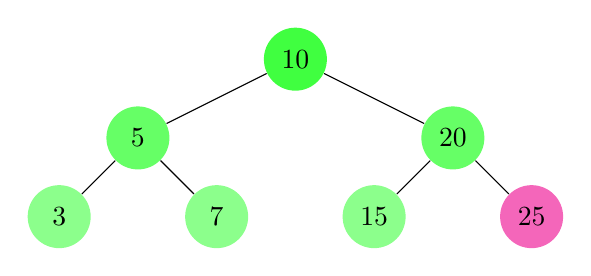
\begin{tikzpicture}[level distance=10mm]
        \tikzstyle{every node}=[fill=green!75,circle,inner sep=1pt, minimum size=8mm]
        \tikzstyle{level 1}=[sibling distance=40mm, set style={{every node}+=[fill=green!60]}]
        \tikzstyle{level 2}=[sibling distance=20mm, set style={{every node}+=[fill=green!45]}]
        \node {10} child {node {5} child {node {3} } child {node {7} }} child {node {20} child {node {15} } child {node[fill=magenta!60] {25} }};
    \end{tikzpicture}
    \caption{Initial Tree Structure}
\end{minipage}
\vspace{1cm}
\end{figure}

\newpage
\subsection*{Search Steps}
Each step below represents a node comparison during the search operation. The tree is visualized at each step, and the current node being compared to the target is highlighted. If the target node is found, it is highlighted in \textcolor{magenta}{magenta}.

\begin{figure}[h!]
\centering
\begin{minipage}{0.8\textwidth}
    \centering
    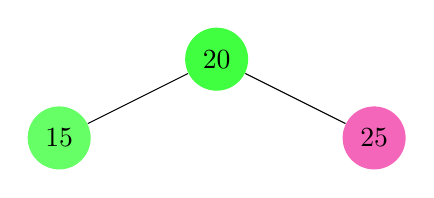
\begin{tikzpicture}[level distance=10mm]
        \tikzstyle{every node}=[fill=green!75,circle,inner sep=1pt, minimum size=8mm]
        \tikzstyle{level 1}=[sibling distance=40mm, set style={{every node}+=[fill=green!60]}]
        \tikzstyle{level 2}=[sibling distance=20mm, set style={{every node}+=[fill=green!45]}]
        \node {20} child {node {15} } child {node[fill=magenta!60] {25} };
    \end{tikzpicture}
    \caption{Step 1: Node comparison}
\end{minipage}
\vspace{1cm}
\end{figure}

\begin{figure}[h!]
\centering
\begin{minipage}{0.8\textwidth}
    \centering
    
\begin{tikzpicture}[level distance=10mm]
        \tikzstyle{every node}=[fill=green!75,circle,inner sep=1pt, minimum size=8mm]
        \tikzstyle{level 1}=[sibling distance=40mm, set style={{every node}+=[fill=green!60]}]
        \tikzstyle{level 2}=[sibling distance=20mm, set style={{every node}+=[fill=green!45]}]
        \node[fill=magenta!60] {25} ;
    \end{tikzpicture}
    \caption{Step 2: Node comparison}
\end{minipage}
\vspace{1cm}
\end{figure}

\newpage
\end{document}
